\subsection{Properties}
\begin{definition}
    Structurally balanced, i.e., \( h = O(\log n) \). RBT is a BST with the following properties:
    \begin{itemize}
        \item Every node is either red or black.
        \item The root is always black.
        \item A red node has only black children.
        \item For all path from root to leaf, there is the same number of black nodes.
        \begin{itemize}
            \item \textbf{Generalizable:} Any node to leaf has the same number of black nodes. 
        \end{itemize}
    \end{itemize}
\end{definition}

\subsubsection{Black height}
\begin{definition}
    The black height \( bh(x) \) is the number of black nodes on any path to a leaf, excluding \( x \).
    \customFigure[0.5]{00_Images/RBT.png}{Red black trees.}
\end{definition}

\subsection{Balancing proof:}
\begin{theorem}
    A RBT with \( n \) internal nodes has 
    \begin{equation}
        h \leq 2 \log(n+1) = O(\log n)
    \end{equation}
\end{theorem}

\begin{theorem}
    \textbf{Lemma:} A subtree in a Red-Black Tree rooted at \( x \) has \textbf{at least}
    \begin{equation}
        2^{bh(x)} - 1
    \end{equation}
    internal nodes.
\end{theorem}

\begin{derivation}
    We will use induction on the height \( h \) of RBT to prove the theorem that \( h \leq 2 \log(n+1) = O(\log n) \), where \( n \) is the number of internal nodes.
    \vspace{1em}

    \begin{enumerate}
        \item \textbf{Basis:} 
        For \( h = 0 \) (i.e. only the root), the tree consists of only one node, which must be black by definition of a red-black tree. The black height of this node is \( bh(\text{node}) = 0 \) (ie. black height excludes the node $x$), so the tree contains no internal nodes:
        \[
        2^0 - 1 = 0 
        \]
        \vspace{1em}

        \item \textbf{Induction Hypothesis:} 
        Assume the lemma holds for all red-black trees with height \( \leq h-1 \). Specifically, assume that such trees have at least \( 2^{bh(x)} - 1 \) internal nodes.
        \begin{itemize}
            \item \( x \) is the root of the subtrees
            \item \( n \) denotes the number of internal nodes.
        \end{itemize}

        \item \textbf{Inductive Step:} Prove this for $h$.
        \vspace{1em}

        Consider a node \( x \) in the tree. We distinguish two cases based on the color of \( x \):
        \begin{itemize}
            \item If \( x \) is red, then the child of $x$ is black, therefore the height of the child (excluding the child) is
            \[
            bh(\text{x.child}) = bh(x) - 1
            \]
            \item If \( x \) is black, the black height of \( x \) is the same as that of its child:
            \[
            bh(\text{x.child}) = bh(x)
            \]
        \end{itemize}

        \customFigure[0.5]{00_Images/IS.png}{The triangles denote subtrees of $h-1$, then adding one node up top with another subtree completes a tree of height $h$. If the root is red, then its children must be black, but not the other way around.}
        \begin{itemize}
            \item \textbf{Key:} We assume here that \( x \) is red, b/c we take take the smallest number since it's \textbf{at least} in the lemma.
        \end{itemize}
        
        \vspace{1em}
        
        Now using this, to compute the \textbf{minimum number of internal nodes} contributed by the \( x \)'s subtrees, where $x$ is the node the at the root's children, we calculate:


        \begin{align*}
            & \text{From the left subtree:} \quad 2^{bh(x)-1} - 1, \\
            & \text{From the right subtree:} \quad 2^{bh(x)-1} - 1, \\
            & \text{Adding the internal nodes of the root's two children:} \quad + 2.
        \end{align*}
        
        Therefore, the total number of internal nodes from both subtrees, plus the contribution of the two children, is given by:
        \[
        2(2^{bh(x)-1}) \leq 2^{bh(x)} \geq 2^{bh(x)-1}
        \]
        \vspace{1em}

        This completes the inductive step, showing that the number of internal nodes for a tree of height \( h \) follows the given bound.
        \vspace{1em}

        \item \textbf{Conclusion: Return to the theorem.} 
        From the lemma, we know that:
        \[
        n \geq 2^{bh(\text{root})} - 1,
        \]
        where \( n \) is the number of internal nodes in the entire tree. This establishes that the tree contains at least \( 2^{bh(x)} - 1 \) internal nodes.
        \vspace{1em}

        In addition, we know that $bh(\text{root}) \geq \frac{h}{2}$, therefore,
        \begin{equation*}
            n \geq 2^{bh{\text{root}}} - 1 \iff n + 1 \geq 2^{h/2} \iff h \leq 2 \log(n+1) = O(\log n) 
        \end{equation*}
    \end{enumerate}
\end{derivation}

\subsection{Rotations in a BST}
\begin{intuition}
    \textbf{Key Properties:}
    \begin{itemize}
        \item \textbf{Preserves BST Property:} Rotations are used to maintain balance without jeopardizing the BST order property. A rotation is a local operation on a BST that preserves the in-order sequence of the nodes.
        \item \textbf{Black-Height Invariance:} In red-black trees, rotations are crucial to maintain the black-height rule. When performed correctly, rotations ensure that the number of black nodes on any path from the root to the leaves remains the same.
    \end{itemize}
\end{intuition}

\subsubsection{Right rotation}
\begin{definition}
    \textbf{Right Rotation:}
    A right rotation is performed on a node \( x \) when its left child \( y \) becomes the new root of the subtree. After rotation, \( x \) becomes the right child of \( y \). This rotation maintains the BST property.

    \[
    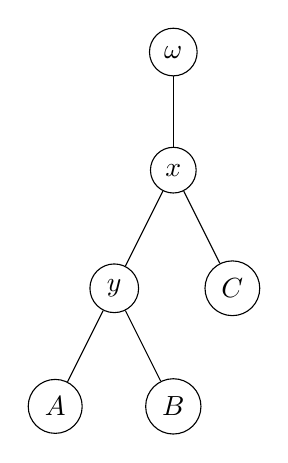
\begin{tikzpicture}[every node/.style={circle,draw},level distance=1.5cm, sibling distance=1.5cm]
    \node (w) {$\omega$}
        child {node (x) {$x$}
            child {node (y) {$y$}
                child {node (A) {$A$}}
                child {node (B) {$B$}}
            }
            child {node (C) {$C$}}
        };
    \end{tikzpicture}
    \quad
    \longrightarrow
    \quad
    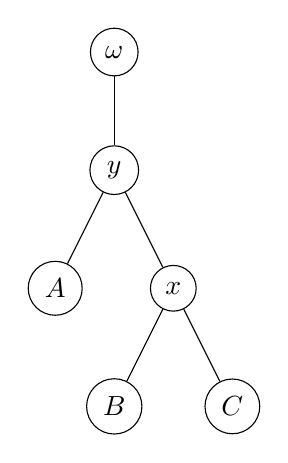
\begin{tikzpicture}[every node/.style={circle,draw},level distance=1.5cm, sibling distance=1.5cm]
    \node (w) {$\omega$}
        child {node (y) {$y$}
            child {node (A) {$A$}}
            child {node (x) {$x$}
                child {node (B) {$B$}}
                child {node (C) {$C$}}
            }
        };
    \end{tikzpicture}
    \]
\end{definition}

\begin{intuition}
    When we pivot around the link from \( x \) to \( y \), we make \( y \) the new root of the sub-tree and \( x \) becomes \( y \)'s right child, and \( y \)'s right child becomes \( x \)'s left child.
\end{intuition}

\subsubsection{Left rotation}
\begin{definition}
    \textbf{Left Rotation:}
    A left rotation is performed when a node \( y \) to become the left child of its right child \( x \). 

    \[
    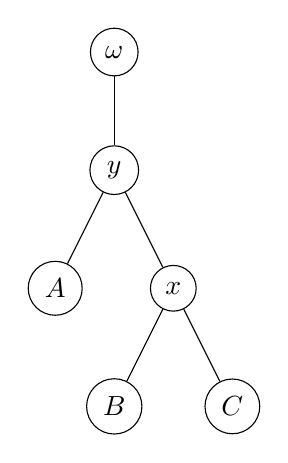
\begin{tikzpicture}[every node/.style={circle,draw},level distance=1.5cm, sibling distance=1.5cm]
    \node (w) {$\omega$}
        child {node (y) {$y$}
            child {node (A) {$A$}}
            child {node (x) {$x$}
                child {node (B) {$B$}}
                child {node (C) {$C$}}
            }
        };
    \end{tikzpicture}
    \quad
    \longrightarrow
    \quad
    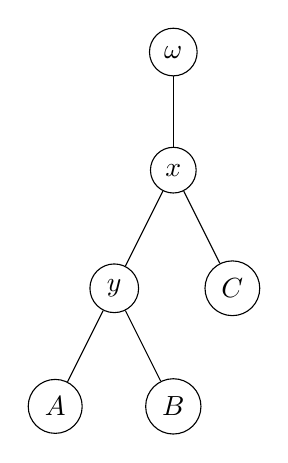
\begin{tikzpicture}[every node/.style={circle,draw},level distance=1.5cm, sibling distance=1.5cm]
    \node (w) {$\omega$}
        child {node (x) {$x$}
            child {node (y) {$y$}
                child {node (A) {$A$}}
                child {node (B) {$B$}}
            }
            child {node (C) {$C$}}
        };
    \end{tikzpicture}
    \]
\end{definition}

\begin{intuition}
    When we pivot around the link from \( y \) to \( x \), we make \( x \) the new root of the sub-tree and \( y \) becomes \( x \)'s left child, while \( x \)'s left child becomes \( y \)'s right child.
\end{intuition}

\subsection{Insert operation}
\begin{process}
    Insert as a leaf (i.e. normal BST) and paint it red. If parent is also red then fix it by rotations. 
    \begin{itemize}
        \item Use rotation and recoloring (i.e. changing the colour of the notes) to do the balancing.
    \end{itemize}
\end{process}

\begin{intuition}
    \begin{itemize}
        \item \textbf{Paint red:} To not jeopardize black height rule but may violate (no two reds rule), but use rotations to shift things around. 
    \end{itemize}
\end{intuition}

\subsubsection{RBT Insert Cases DONT UNDERSTAND THIS}
\begin{definition} Say we are inserting $x$, then 

    \textbf{Cases 1-3:} If $p(x)$ (i.e. parent of x) is the left child of $p(p(x))$ (i.e. parent of parent of x).
    \textbf{Cases 4-6:} If $p(x)$ (i.e. parent of x) is the right child of $p(p(x))$ (i.e. parent of parent of x).
    \begin{itemize}
        \item If root becomes red, paint it black. 
    \end{itemize}

    \begin{itemize}
        \item  \textbf{Case 1,4: Sibling \( y \) of \( p(x) \) is red}
        \customFigure[0.75]{00_Images/C1.png}{C1}

        \item \textbf{Case 2: Sibling \( y \) of $p(x)$ is black, \( x \) is the right child}
        \customFigure[0.75]{00_Images/C2.png}{C2}

        \item \textbf{Case 3: Sibling \( y \) of $p(x)$ is black, \( x \) is the left child}
        \customFigure[0.75]{00_Images/C3.png}{C3}
    \end{itemize}
\end{definition}